\begin{figure*}[htbp!]
	\centering
	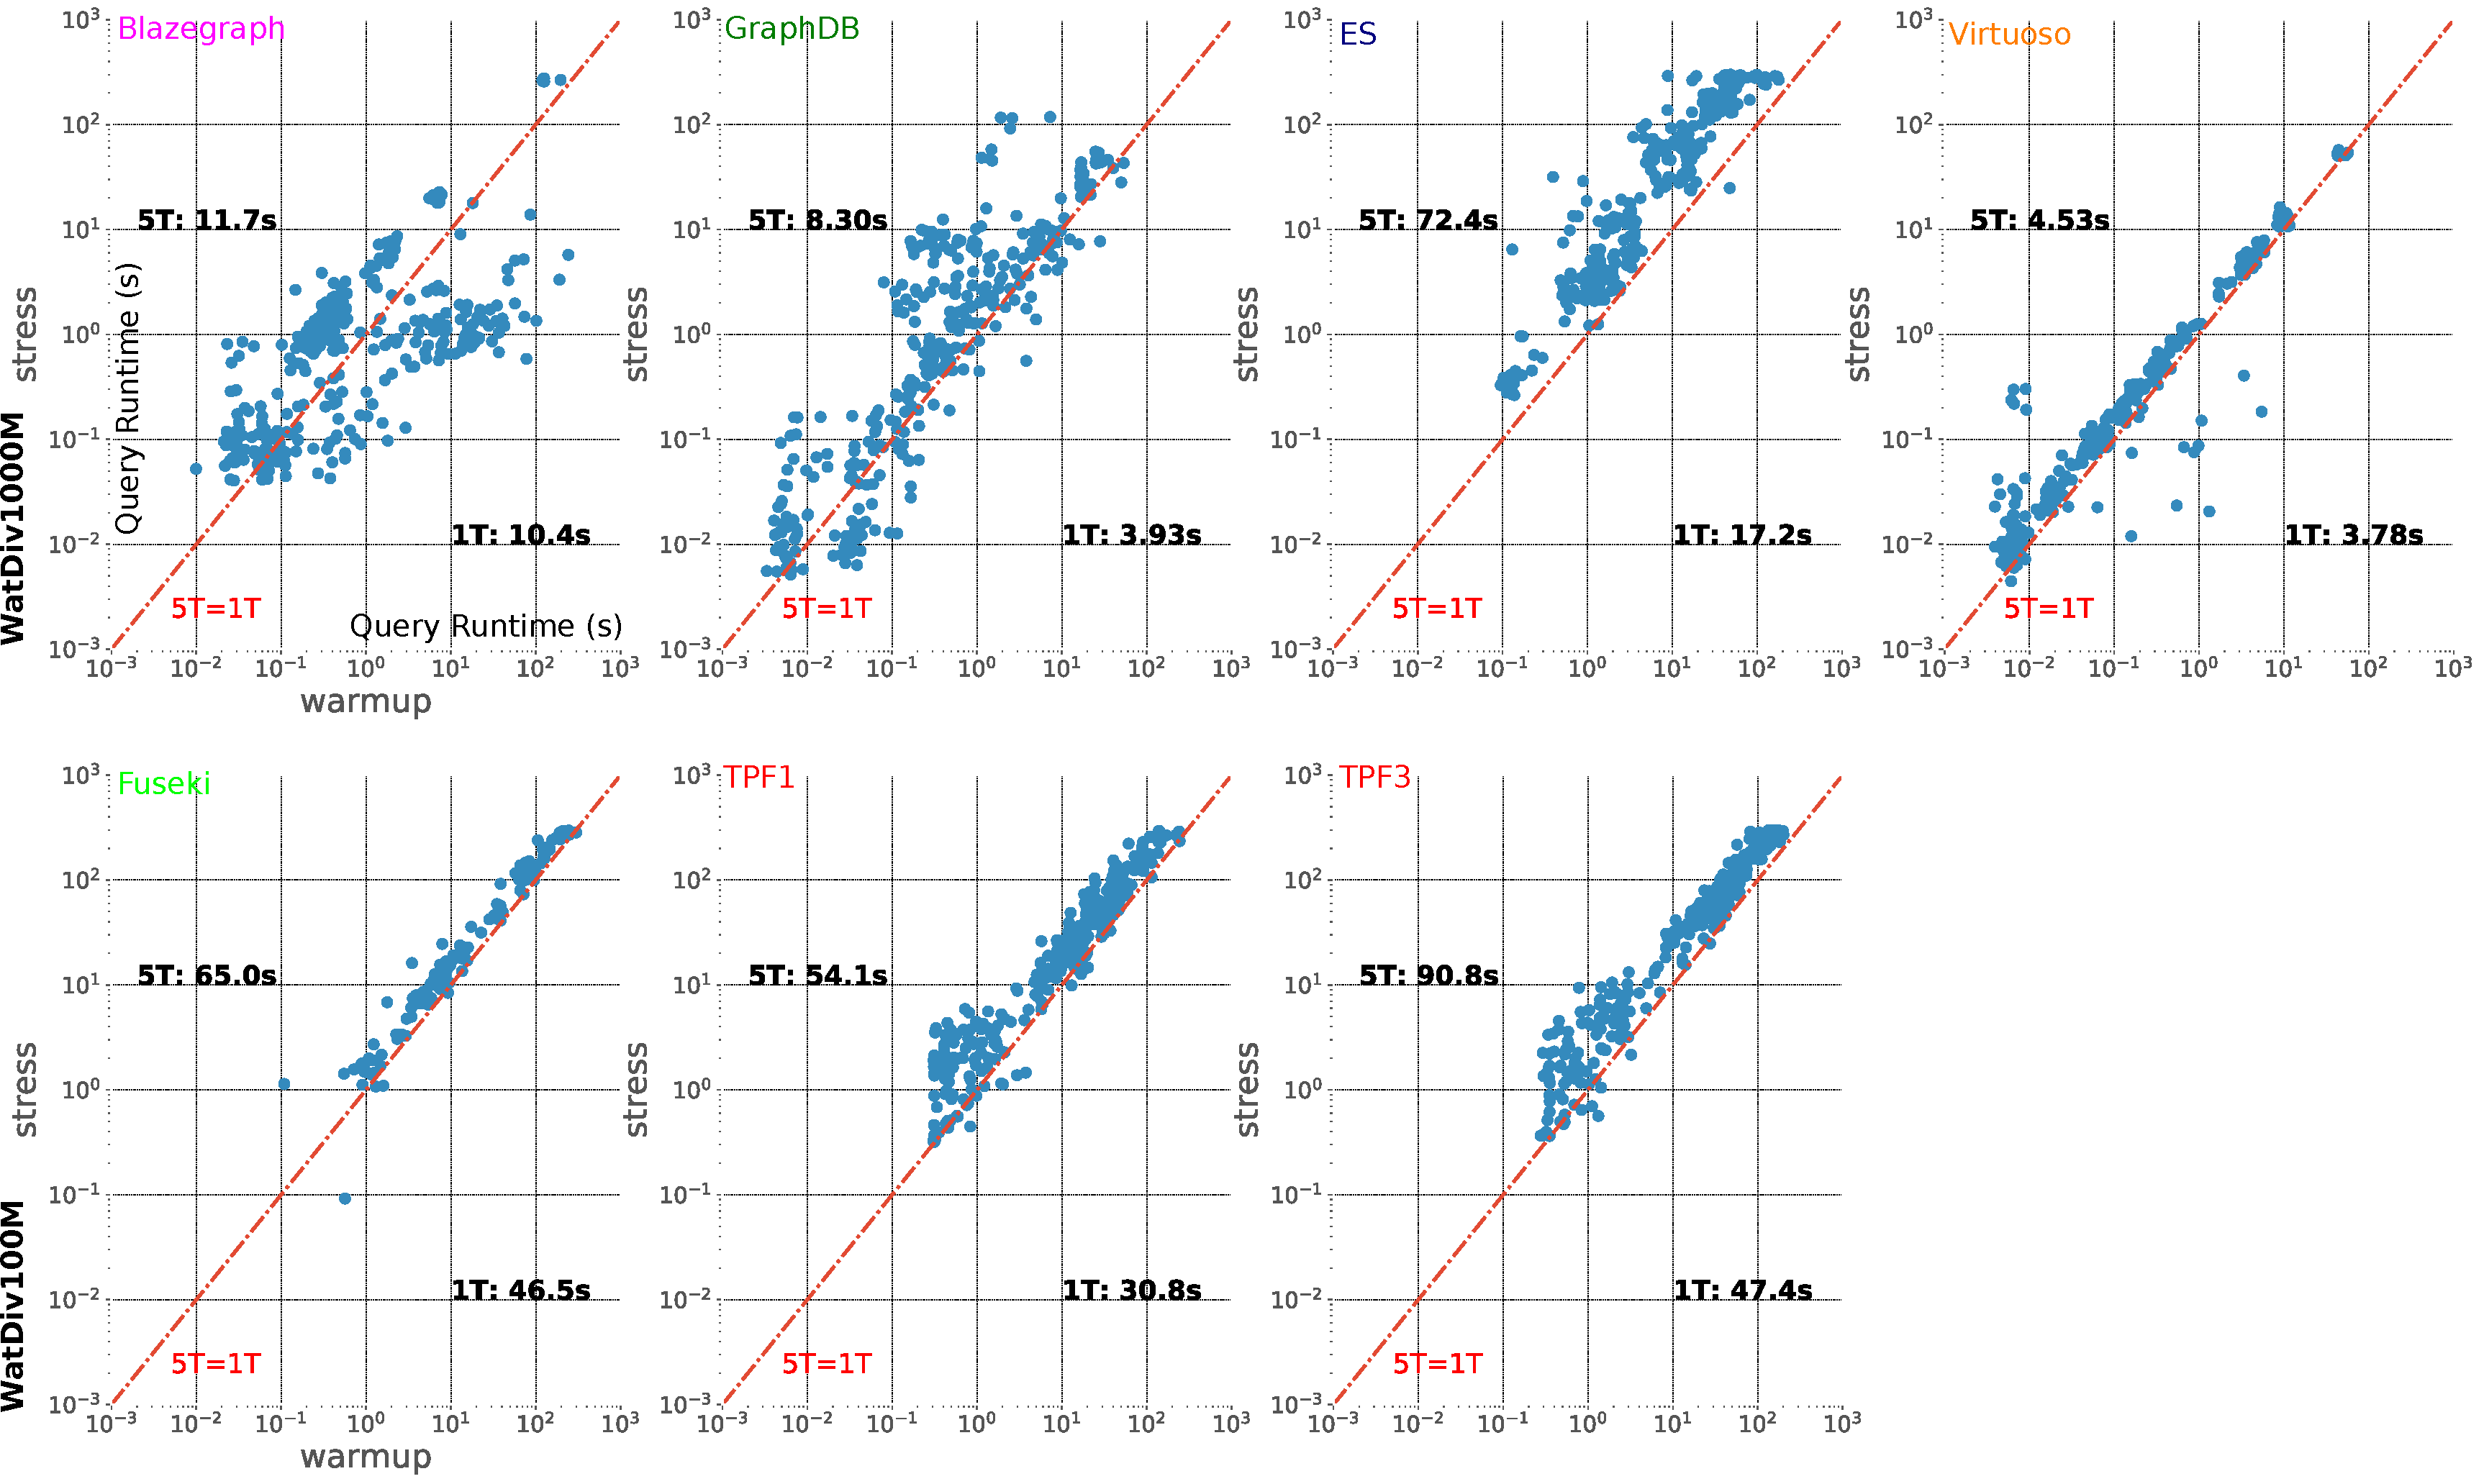
\includegraphics[width=0.90\linewidth]{imgs/Fig07_Watdiv_SingleMultiClient}
	\caption{Runtimes for single versus multi-client workloads: 1 vs. 5 threads. 
		5T runtime corresponds to the maximum runtime per query in the stress test, 1T is the runtime during the warm-up phase. The red line corresponds to the bisector, where the runtime for both workloads is equal. Dots are expected to be shifted up, which correspond to a multiplication factor. The closer the dots to the bisector the smaller the multi-client overhead. Dots below the bisector can be attributed to the natural variance in query runtimes. Average runtimes per store are also shown. \textbf{Bla1\_64} and \textbf{Vir1\_64} have the smallest overhead $(< 20\%)$, for \textbf{ES1\_64} has the largest $(> 300\%)$.
	}
	\label{fig:Fig07_Watdiv_SingleMultiClient}
\end{figure*}
%
%RESULTS Rev1: Notebook Rev1_11 
%results
%1T vs 5T are the runtime of the MEAN query!
%5T runtime corresponds to the max runtime of a query in the stress test, 1T is the runtime during the warmup phase, 5T was chosen max to try and suppress caching effects, therefore fluctuations might be mainly attributed to gaussian noise
%FIGure Caption
%Runtimes for single versus multi-client workloads: 1 vs. 5 threads. 
%5T runtime corresponds to the maximum runtime per query in the stress test, 1T is the runtime during the warmup phase. The red line corresponds to the bisector, where the runtime for both workloads is equal. Dots are expected to be shifted up, which correspond to a multiplication factor. The closer the dots to the bisector the smaller the multi-client overhead. Dots below the bisector can be attributed to the natural variance in query runtimes. Average runtimes per store are also shown. \textbf{Bla1\_64} and \textbf{Vir1\_64} have the smallest overhead $(< 20\%)$, for \textbf{ES1\_64} has the largest $(> 300\%)$.
All results so far focused on the multi-threaded benchmark run, in which 5 benchmark clients are simultaneously executing the same query-mix in a (different) randomized order. It is however interesting to take into account the effect of server load. In Figure~\ref{fig:Fig07_Watdiv_SingleMultiClient} we compare, per query, the runtime of the warm-up run versus the runtime of the slowest multi-threaded run. We chose the slowest query as this has the highest probability of eliminating the effects of caching which will be studied in the next section. Note that for the \emph{SemWeb} systems the comparison is on WatDiv100M, while the \emph{Vendor} systems are compared on WatDiv1000M.

%Bla, Gra, ES, Vir, Fus, TPF1, TPF3
%11.7	10.4		1.125
%8.3	3.93		2.1119592875
%72.4	17.2		4.2093023256
%4.53	3.78		1.1984126984
%65		46.5		1.3978494624
%54.1	30.8		1.7564935065
%90.8	47.4		1.9156118143

\begin{itemize}
	\item \textbf{Highest resilience against server loads}: The lowest multiplication factors (mf) are 1.1 , 1.2, and 1.4 for \textbf{Vir1\_64\_Opt}, \textbf{Bla1\_64\_Opt}, and \textbf{Fus1\_64\_Def} respectively. 
	 
	\item \textbf{Lowest resilience against server loads:} For \textbf{TPF*\_64\_Def} the mf is 1.8 - 1.9.  \textbf{Gra1\_64\_Opt}'s mf is at 2.1, but for \textbf{ES1\_64\_Opt} we have an mf of 4.2.
	
	\item \textbf{Variance of query runtimes:} For Blazegraph and GraphDB the variance on the query runtimes might still be explained as the result of caching. As we will see in the next section however, caching only plays a role for the slow-running queries (\textbf{C}-templates) in the case of Blazegraph.
\end{itemize}
